%============================================================================%
% Author: Pablo S�nchez                                                      %
%         p.sanchez@unican.es, http://personales.unican.es/sanchezbp         %
% Section : validating                                   Date: 28/02/2011    %
% Version : 1.0                                                              %
% Conference: SPLC 2011                                                      %
%============================================================================%

Once we have specified a set of cross-tree constraints for a feature model including clonable feature, we might want, and we should, to analyse them. The most basic and required analysis operation is to decide when a given configuration is a valid configuration, i.e. it satisfies all the specified constraints. Nevertheless, other analysis operations, such as the ones surveyed for Benavides et al~\cite{Benavides:2010}, are of interest. An example of this operation are the analysis of \emph{promising partial configuration} and \emph{dead features}.
The \emph{promising partial configuration} analyses if a partial configuration satisfies the constraints and
the features for which a decision have not been adopted yet can be assigned a value in way that all the constraints are satisfied. The \emph{dead features} analysis consist on checking if each feature can be included in one valid configuration at least. Otherwise, such a feature might not have been selected, so it would not make sense to have it included in the feature model. Dead features are symptoms of ill-designed feature models.
The input for this analysis process

To be able to carry out this kind of analysis, the expressions constructed using the language presented in the previous section are transformed into a Constraint Satisfaction Problem~\cite{tsang:1993}. We have opted for this formalism due to the reported advantages~\cite{Benavides:2010}, as well as for the good performance provided by the Choco library for CSP solving~\cite{rochart:2008}.

A Constraint Satisfaction Problem is defined as a tuple $(X, D, C)$, where $X$ is a finite set of variables, $D$ is a finite set of domains of values (one domain for each existing variable in $X$), and $C$ is set of constraints defined on $V$. Thus, the steps to transform our constraint set into a CSP are: (1) to decide how many variables we have to create; (2) what the domains for these variables are; and (3) how to transform the constraints to express them properly as constraint for a CSP.

%================================================================================================================
% NOTE(Pablo): This is disturbing and breaks the flow of the paper
%================================================================================================================
%
% A first tentative, is to create a variable by each potential feature, and to assign to each variable a boolean
% value depending on if the variable has been selected or not. Nevertheless, since clonable features can have an
% infinite upper bound, there might be an infinite number of variables, and the set of variables $X$ must be finite. % But, it should be noticed that although a feature model can have an  infinite number of configurations, each
% configuration is finite, since each configuration must have, by definition, a finite number of clones. Therefore, % clonable and multiple features are translated into variables of a CSP based on a (partial) configuration model,
% instead of a configuration model.
%
%================================================================================================================

For the transformation process, all features will be considered as clonable features. Mandatory ones will have  a $[1..1]$ multiplicity; whereas optional ones will have $[0..1]$. Feature groups, which have not been used for the Smart Home case study, are transformed into a set of optional features plus a set of cross-tree constraint for ensuring group cardinality, as usual in the literature~\cite{czarnecki:2005sc}.

Before creating the variables, the \emph{real lower and upper bound} for each feature are calculated. We say \emph{real} because a feature can have more instances than the upper bound of its multiplicity. Similarly, a feature can have less instances than the lower bound of its multiplicity. Figure~\ref{fig:lowerUpperBounds} illustrates this situation. In Figure~\ref{fig:lowerUpperBounds} (a), the feature \imp{C} has as upper bound 2, which means it can appear two times per instance of the feature \imp{B} as a maximum. But in the context of the whole feature model, feature \imp{B} can appear three times as a maximum, so there can be a maximum of six instances of feature \imp{C} per feature model. This would be the \imp{real upper bound} of feature \imp{C}. The \emph{real upper bound} can be defined as the maximum number of instances of a feature in a configuration model as a whole, instead of in a per feature basis.

Similarly, the lower bound for feature {C} is 1, which means there must be one instance at least per instance of the feature \imp{B}. Nevertheless, since feature \imp{B} might have zero instances, it would possible to create a configuration model with zero instances of the feature {C}. So, zero would be the \emph{real lower bound} of feature \imp{C}. The \emph{real lower bound} can be defined as the minimum number of instances of a feature in a configuration model as a whole, instead of in a per feature basis.

The real upper bound of a feature $F$ is calculated by multiplying the upper bounds of each feature in the path from such a feature $F$ to the root of the feature model. It should be noticed as soon as the upper bound of a feature in this path is infinite, the real upper bound of the feature $F$ will be infinite. This would be the case for feature $C$ in Figure~\ref{fig:lowerUpperBounds} (b). Similarly, the real lower bound of a feature $F$ is calculated by multiplying the lower bounds of each feature in the path from such a feature $F$ to the root of the feature model. It should be noticed as soon as the lower bound of a feature in this path is zero, the real lower bound of the feature $F$ will be zero. This would be the case for feature $C$ in Figure~\ref{fig:lowerUpperBounds} (a) and (b).

\begin{figure}
  % Requires \usepackage{graphicx}
  \centering 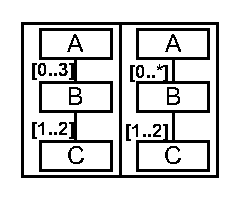
\includegraphics[width=.3\linewidth]{Figures/lowerUpperBounds.eps}\\
  \caption{Calculating lower and upper bound of clonable features}
  \label{fig:lowerUpperBounds}
\end{figure}

The algorithm for creating the variables for the CSP is as follows:

\begin{enumerate}
	\item A variable for each feature in the feature model is created. If the feature can be univocally identified, the name of the variable is the same name as the name of the feature. Otherwise, we preclude the name of the variable with the names of as many ancestor features as required to univocally identified it. For instance, the feature \imp{LightMng} below \imp{GeneralFacilities} would be named as \imp{GeneralFacilities\_LightMng}.
	\item The real upper bound for each feature is calculated.
	\item The domain $[a - b] \in \mathds{N}$ is associated to each variable. $a, b$ are positive integers (including zero), $b$ can be infinite and $a \leq b$. $a$ is the lower bound of the multiplicity corresponding to the feature the variable represents, and $b$ is the real upper bound for such a feature.
	\item For each instance of clonable feature in a given configuration model, a new variable is created. The domain for these variables is $1 \in \mathds{N}$. The name of the clone is used as name for the variable. Each clone must be given a unique name (this must be ensured by the feature modelling tool).
	\item For each instance of a multiple feature in a given configuration model, a new variable is also created. The domain for these variables is $[a - b] \in \mathds{N}$, where $a$ and $b$ are the \emph{real lower and upper bounds} for that feature, but using as root the nearest clone in the path to the root. The name of the variable is the name of the feature preceded by the name of the first clone found in the path from the multiple feature to the root of a configuration model.
	\item Finally, we need to bind the variables that have been already selected or unselected in the configuration model. For each boolean variable $v$, a constraint \imp{eq(v,true)} is added to the set of constraints if the corresponding feature has been selected; otherwise, a constraint \imp{eq(v,false)} is added to such a set. For each integer variable representing a clonable or multiple feature, the number of clones is calculated and that variable initialized to that number of clones.
\end{enumerate}

%=============================================================================================================%
% NOTE(Pablo): This is boring, so I have simply skipped them
%=============================================================================================================%
%
% Applying this process to the feature model of Figure~\ref{fig:smartHomeFM} and the configuration model of
% Figure~\ref{fig:smartHomeCfg} would be as follows:
%
% \begin{enumerate}
%    \item We create a variable for $SmartHome$ and $Facilities$ with domain ${true,false}$.
%    \item We create the variables $Floor$, $Room$, $Devices$, $FloorFacilities$, $RoomFacilities$ with domain
%     $[1..*]$.
%    \item We create the variables $Window$, $Heater$ and $Light$, $LightMng$,
%          $WindowMng$, $HeaterMng$ and $SmartEnergyMng$ with domain $[0..*]$.
%    \item We create the variables $Facilities_LightMng$, $Facilities_WindowMng$, $Facilities_LightMng$ and
% $Facilities_SmartEnergyMng$ with domain ${true,false}$.
%    \item We create the variables $GroundFloor_FloorFacilities$, $GroundFloor_FloorFacilities_WindowMng$,
% $GroundFloor_FloorFacilities_LightMng$ and $GroundFloor_FloorFacilities_SmartEnergyMng$ with domain
% ${true,false}$.
%    \item We create the variables $GroundFloor_Room$, $GroundFloor_RoomFacilities$, $GroundFloor_Devices$ with
% domain $[1..*]$.
%    \item We create the variables $GroundFloor_Window$, $GroundFloor_Heater$, $GroundFloor_Light$,
% $GroundFloor_LightMng$, $GroundFloor_WindowMng$, $GroundFloor_HeaterMng$ and $GroundFloor_SmartEnergyMng$ with
% domain $[0..*]$.
%    \item We create the variables $Kitchen_RoomFacilities$, $Kitchen_RoomFacilities_WindowMng$,
% $Kitchen_RoomFacilities_LightMng$ and $GroundFloor_RoomFacilities_SmartEnergyMng$ with domain ${true,false}$.
%
%    \item We create the variables $Kitchen_Window$, $Kitchen_Heater$, $Kitchen_Light$ with domain $[0..*]$.
%    \item We create similar variables to steps 8 and 9, but for the \imp{Bedroom} clone.
% \end{enumerate}

Once we have created the variables and the domains, the remaining step is to express the constraints in a suitable form for being managed as a CSP. We would need to express these constraints in Choco syntax. Choco is the third-party Java library we have selected for CSP solving due to the promising performance it has shown in several benchmarks~\cite{rochart:2008}. Choco provides logical operators plus comparison operators for specifying constraints. Thus, the problem of translating logical expressions and comparison expressions can be reduced to rewriting the constraints specified in the language presented in the previous section in proper Choco syntax.

%=============================================================================================================%
% NOTE(Pablo): This is considered trivial and left out of the paper
%=============================================================================================================%
%
% \begin{figure}
% \begin{scriptsize}
% \begin{verbatim}
%    \imp{implies(Facilities\_SmartEnergy,and(Facilities\_HeaterMng,Facilities\_WindowMng))}
% \end{verbatim}
% \end{scriptsize}
% \caption{CSP constraint for constraint \imp{C01}}
% \label{eq:c01}
% \end{figure}
%
%=============================================================================================================%

Thus, our problem is basically reduced to the translation of context expressions. The solution for this case is to create a new constraint for each clone which serves as context for a expression or subexpression. The new constraint is rewritten for that particular context. For instance, constraint \imp{CO1} (see Figure~\ref{fig:constraints}) would be rewritten as shown in Figure~\ref{fig:c01}.

\begin{figure}
\begin{footnotesize}
\begin{center}
\texttt{GeneralFacilities\_SmartEnergyMng implies (GeneralFacilities\_HeaterMng and GeneralFacilities\_WindowMng)}.
\end{center}
\end{footnotesize}
\caption{Constraint \imp{C01} rewritten in Choco syntax}
\label{fig:c01}
\end{figure}

If quantifiers are used, the generated constraints are connected by \emph{and} or \emph{or} operators depending on if the \imp{all} or the \imp{any} quantifier has been used. For the cases where a context expression evaluates to a positive integer, we simply count how many generated constraints are satisfied.

%=============================================================================================================%
% NOTE(Pablo): It has been written in a more user-friendly way
%=============================================================================================================%
%
% translating a constraint like \imp{<quantifier> <MultiValueFeature> [ Constraint ]}, is to replicate the
% translation of \imp{<Constraint>} as many times as clones the \imp{<MultiValueFeature>} has. The translation of
% \imp{<Constraint>} is performed as any other constraint, but assuming that each replica of \imp{<Constraint>} is
% evaluated in the context of an unique clone of such a feature, i.e. the constraint is evaluated using exclusively % the subtree below that clone. Therefore, we need to replace the variables in \imp{<Constraint>} by the variables
% that refer to the features below the clone. If the quantifier is \imp{any}, we join all these replicas by
% \emph{or} relationships. If the quantifier is \imp{all}, we join all these replicas by \emph{and} relationships.
%
%
% We denote that a constraint $C$ is evaluated using a given feature instance $FI$ as context as \imp{I \vDash C}.
% Thus, for instance, using the configuration model of Figure~\ref{fig:smartHomeCfg}, $\imp{Kitchen} $\vDash$
% LightMng$} would be evaluated to false, whereas $\imp{Bedroom} $\vDash$ LightMng$} would be evaluated to true.
%
%=============================================================================================================%

For instance, in the case of the constraint \imp{C10} (see Figure~\ref{fig:constraints}) and the configuration model of Figure~\ref{fig:smartHomeCfg}, three constraints would be generated, one per each room instance. These constraints would be rewritten to particularize it for each clone and the they will be connected by \emph{and} operators, as shown in Figure~\ref{eq:c10}

\begin{figure}
\begin{center}
\begin{footnotesize}
\begin{verbatim}
and(implies(Kitchen_SmartEnergy,
	  and(Kitchen_HeaterMng, Kitchen_WindowMng)),
   and(implies(Living_SmartEnergy,
		and(Living_HeaterMng, Living_WindowMng))),
	  implies(Bed_SmartEnergy,
		and(Bed_HeaterMng,Bed_WindowMng)))
\end{verbatim}
\end{footnotesize}
\end{center}
\caption{Constraint \imp{C10} expanded rewritten in Choco syntax}
\label{eq:c10}
\end{figure}

%, would be translated following the next process: (1) We calculate the set of clones of the feature $Floor$. In
% this case, $Floor = {GroundFloor}$. Thus, each feature in the internal constraint refers to a feature below
% $GroundFloor$; (2) Then, we translate the internal constraint, which generates a Choco constraint such as depicted % in~\ref{eq:C05}.
%
% \begin{figure}
% \begin{scriptsize}
% \begin{verbatim}
%  implies(GroundFloor\_FloorFacilities\_SmartEnergy,
%          and(GroundFloor\_FloorFacilities\_HeaterMng,
%              GroundFloor\_FloorFacilities\_WindowMng))}
% \end{verbatim}
% \end{scriptsize}
% \caption{CSP constraint for constraint \imp{C05}}
% \label{eq:c05}
% \end{figure}
%
% In the case of the constraint \imp{C13} in Figure~\ref{fig:constraints}, we would need to create several replicas % of the constraint, and to use different sets of variables for each replica, according to the different clones of
% the feature \imp{Room}. The translation of such a constraint is depicted in Figure~\ref{eq:13}
%
% \begin{figure}
% \begin{scriptsize}
% \begin{verbatim}
%  and(implies(Kitchen_HeaterMng,gt(Kitchen\_Heater,0)),
%             implies(Bedroom\_HeaterMng,gt(Bedroom\_Heater,0))))}
% \end{verbatim}
% \end{scriptsize}
% \caption{CSP constraint for constraint \imp{C05}}
% \label{eq:c13}
% \end{figure}

Once we have defined our CSP, we can solve it using a third-party library as Choco. Choco calculates if the current configuration satisfies the external constraints, and if it is not so, it provides information about what constraints has been violated. Moreover, Choco can be used to perform some kind of useful analysis on partial configurations, calculating if exist one solution at least for the given CSP. This is useful to analyse when a partial configuration is promising, i.e. when it is part of a valid product. It can be also used to perform \emph{dead features analysis}. For each feature, we would calculate if there is one solution at least for the CSP problem with such a feature selected. If this solution is found, the feature is included in at least one valid product. Otherwise, that feature can not be selected and it is considered dead.

Next section comments on the experiments we have carried out for validating our approach and discuss briefly on strengths and weaknesses.

% For instance, given an invalid partial configuration, Choco can use constraint propagation to calculate what
% features should be added to the current configuration in order to create a valid configuration. We can also Choco % to complete a configuration given a certain criteria.

% For instance, let us suppose we have the configuration model of Figure~\ref{fig:smartHomeCfg}, but \imp{WindowMng} % has not been selected neither at the \imp{Floor} nor at the \imp{Room} level (and it has been selected at the
% house level). But, according to constraints \imp{C02} and \imp{C07}, it should have been also selected at the
% floor and room levels. Using constraint propagation, Choco can calculate that these features are lacking at these % levels, and \emph{Hydra}, our feature modelling tool, would add them to the configuration model.

% If, given a partial configuration, this can be completed in several ways, we can use Choco to select the
% configuration, which fulfill some kind of arbitrary criteria, such as having the lower number of features.


%=============================================================================================================%
% NOTE(Pablo): It has been written in a more user-friendly way
%=============================================================================================================%
%
% In our case, $V$ would be the features contained in the feature model. Each simple feature is transformed into a
% variable $v \in V$, with domain $D_{i} = {TRUE, FALSE}$. Each clonable and multiple feature is transformed into a
% variable $v \in V$ with domain $D_{i} = {a..b}$, where $a$ is the minimum number of times the clonable feature
% can
% appear in a feature diagram and $b$ the upper bound. These limits do not necessarily need to be the limits of the
% clonable feature. See for instance, Figure~\ref{fig:lowerUpperBounds} (a). Feature \imp{D} has as lower bound $1$, % but % it means it need to appear $1$ time by each feature $B$, and there must be $4$ clones of the feature $B$ at % least.
% Therefore, the minimum number of clones of the feature $D$ in a whole configuration model is $4$. The global
% lower bound of a feature $F$ is calculated by multiplying the lower bounds of each feature in the path from such a % feature
% $F$ to the root of the feature model. In this path, optional features are considered to have cardinality $0..1$,
% mandatory features $1..1$ and grouped features has the same cardinality as the feature group. Upper bounds are
% calculated in the same way, but multiplying the upper bounds of each features. It should be noticed that any $0$
% in the lower bound of the features in that path means the lower bound will be zero, and any $*$ in the upper
% bounds means that the upper bound will be $*$. Then, for each clone in the feature model we create a variable $v
% \in V$. We do not % consider clones the selections of simple features. These variables has as domain ${TRUE}$, it % is said, they always evaluate to true since they already exist in the configuration model.
%
%=============================================================================================================% 